\section{CÁC KHÁI NIỆM MỞ ĐẦU}
\subsection{TÓM TẮT LÝ THUYẾT}
\subsubsection{Khái niệm vectơ}
Cho đoạn thẳng $AB$. Nếu chọn điểm $A$  làm điểm đầu, điểm  $B$ làm điểm cuối thì đoạn thẳng $AB$  có hướng từ $A$  đến $B$. Khi đó ta nói  $AB$ là một \indamm{đoạn thẳng có hướng}.	
		\begin{itemize}
		\item[\iconMT] \indam{ Định nghĩa: }
		\begin{itemize}
			\item  Vectơ là một đoạn thẳng có hướng, nghĩa là trong hai điểm mút của đoạn thẳng đã chỉ rõ điểm đầu, điểm cuối.
			\item  Độ dài vectơ là khoảng cách giữa điểm đầu và điểm cuối của vectơ đó.
		\end{itemize}
		\item[\iconMT]\indam{ Chú ý:}
		\immini{
			\begin{itemize}
			\item Nếu chỉ rõ điểm đầu là $A$ và điểm cuối là $B$, ta có "vectơ $AB$", kí hiệu $\overrightarrow{AB}$. Nếu không cần chỉ rõ điểm đầu và điểm cuối, ta dùng các chữ cái thường để kí hiệu. Ví dụ $\overrightarrow{a}, \overrightarrow{b}, \overrightarrow{x},...$
			\item  Độ dài $\overrightarrow{a}$, kí hiệu $|\overrightarrow{a}|$; Độ dài $\overrightarrow{AB}$, kí hiệu $|\overrightarrow{AB}|$ và hiển nhiên $|\overrightarrow{AB}|=AB$.
			\end{itemize}	}{
	\hspace{2cm}
		\begin{tikzpicture}[smooth,samples=300,scale=0.8,>=stealth,font=\footnotesize]
		\tkzDefPoints{0/0/A,3/1/B}
		\draw[->] (0,0)--(3,1);
		\draw[->] (1,-1)--(4,-1);
		\tkzDrawPoints[size=2,fill=black](A,B)
		\node[below] at (3,-1) {$\overrightarrow{x}$};
		\tkzLabelPoints[below](A)
		\tkzLabelPoints[below right](B)
		\end{tikzpicture}}
	\end{itemize}

\subsubsection{Vectơ cùng phương, cùng hướng}
Đường thẳng đi qua điểm đầu và điểm cuối của vectơ gọi là giá của vectơ đó.
	\begin{itemize}
		\item[\iconMT] Hai vectơ cùng phương nếu giá của chúng song song hoặc trùng nhau.	
		\item[\iconMT] Khi hai vectơ cùng phương, chúng có thể cùng hướng hoặc ngược hướng.
			\begin{center}
			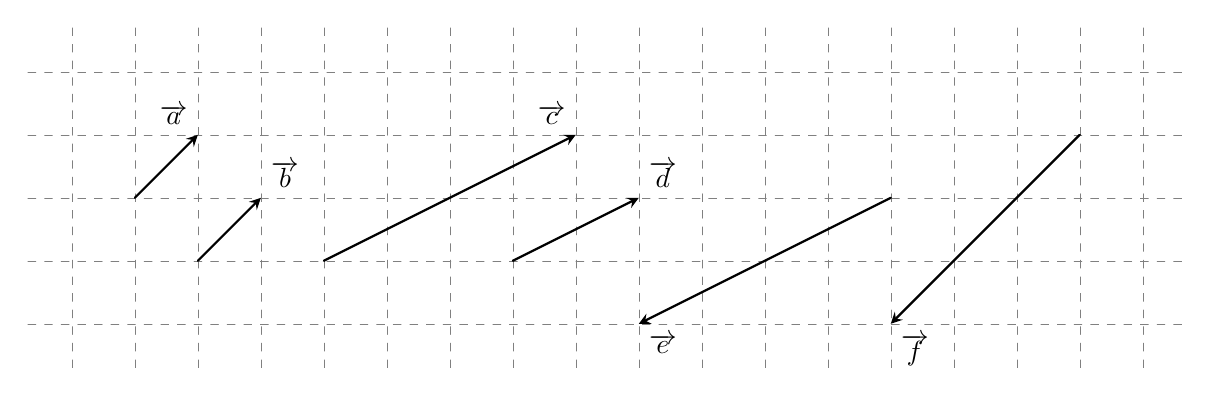
\begin{tikzpicture}[>=stealth,scale=0.8, line join=round, line cap=round]
			\draw[line width=0.05pt,gray,dashed] (-0.7,-0.7) grid (17.7,4.7);
			\draw[->,thick](1,2)--(2,3)node[above left]{$\overrightarrow{a}$};
			\draw[->,thick](2,1)--(3,2)node[above right]{$\overrightarrow{b}$};
			\draw[->,thick](4,1)--(8,3)node[above left]{$\overrightarrow{c}$};
			\draw[->,thick](7,1)--(9,2)node[above right]{$\overrightarrow{d}$};
			\draw[->,thick](13,2)--(9,0)node[below right]{$\overrightarrow{e}$};
			\draw[->,thick](16,3)--(13,0)node[below right]{$\overrightarrow{f}$};
			\end{tikzpicture}
		\end{center}
		Trong hình vẽ trên
		\begin{itemize}
			\item [$\bullet$] các cặp vec tơ cùng phương: $\overrightarrow{a}$ cùng phương $\overrightarrow{b}$; $\overrightarrow{a}$ cùng phương $\overrightarrow{f}$; $\overrightarrow{d}$ cùng phương $\overrightarrow{e}$,...
			\item [$\bullet$] các cặp vec tơ cùng hướng: $\overrightarrow{a}$ cùng hướng $\overrightarrow{b}$; $\overrightarrow{c}$ cùng hướng $\overrightarrow{d}$.
			\item [$\bullet$] các cặp vec tơ ngược hướng: $\overrightarrow{a}$ ngược hướng $\overrightarrow{f}$; $\overrightarrow{c}$ ngược hướng $\overrightarrow{e}$; $\overrightarrow{d}$ ngược hướng $\overrightarrow{e}$;
			\end{itemize}
	\end{itemize}
\subsubsection{Vectơ bằng nhau}
Hai vec tơ $\vec{a}$ và $\vec{b}$ được gọi là bằng nhau, kí hiệu $\vec{a}=\vec{b}$ nếu chúng có cùng hướng và cùng độ dài.
\subsubsection{Vectơ-không}
	\begin{itemize}
		\item[\iconMT] \indam{Định nghĩa: }Là vectơ có điểm đầu và điểm cuối trùng nhau. 
		\begin{itemize}
			\item Kí hiệu $\overrightarrow{0}$, nghĩa là $\overrightarrow{0}=\overrightarrow{AA}=\overrightarrow{BB}$...;
			\item Độ dài vectơ-không bằng $0$, nghĩa là $\bigg|\overrightarrow{0}\bigg|=0$.
		\end{itemize}

		\item[\iconMT]  \indam{Qui ước: }Vec tơ-không cùng phương và cùng hướng với mọi véc tơ.
	\end{itemize}